\subsubsubsubsection{Lane}
\begin{figure}[h]
\centering
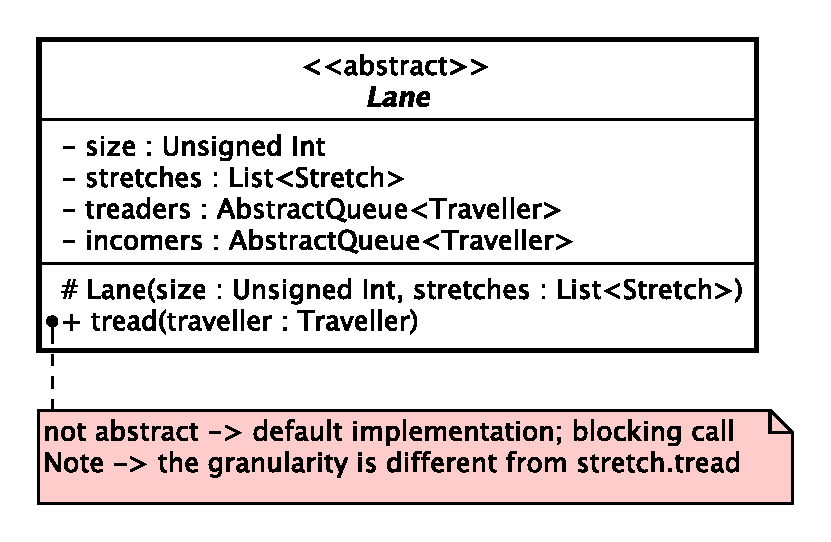
\includegraphics[scale=0.6,keepaspectratio]{images/solution/app/backend/lane.eps}
\caption{\pReactiveComponentLane::Lane}
\label{fig:sd-app-lane}
\end{figure}
\FloatBarrier
\begin{itemize}
  \item \textbf{\descr} \\
    It represents a lane entity. It is a protected object composed of one or
    more stretches.
  \item \textbf{\attrs}
  \begin{itemize}
    \item \texttt{size: Unsigned Int} \\
The size of the stretch/treading queue.
    \item \texttt{stretches: List<Stretch>} \\
The list of stretches which compose the lane.
    \item \texttt{treaders: AbstractQueue<Traveller>} \\
The queue of travellers which are treading the lane.
    \item \texttt{incomers: AbstractQueue<Traveller>} \\
The queue of travellers which are waiting to tread the lane. 
  \end{itemize}
  \item \textbf{\ops}
  \begin{itemize} 
    \item[\#] \texttt{Lane(size: Unsigned Int, stretches: List<Stretch>)} \\
Creates a \texttt{Lane} object with a specific size and list of stretches.
    \item[+] \texttt{tread(traveller: Traveller)} \\
Implements the lane treading. Moves the traveller on the stretches which are 
in the traveller route.
  \end{itemize}
\end{itemize}
